\section{Federated Truth Discovery: Overview and Key Issues}

\subsection{Overall Design}

\begin{figure}
	\centering
	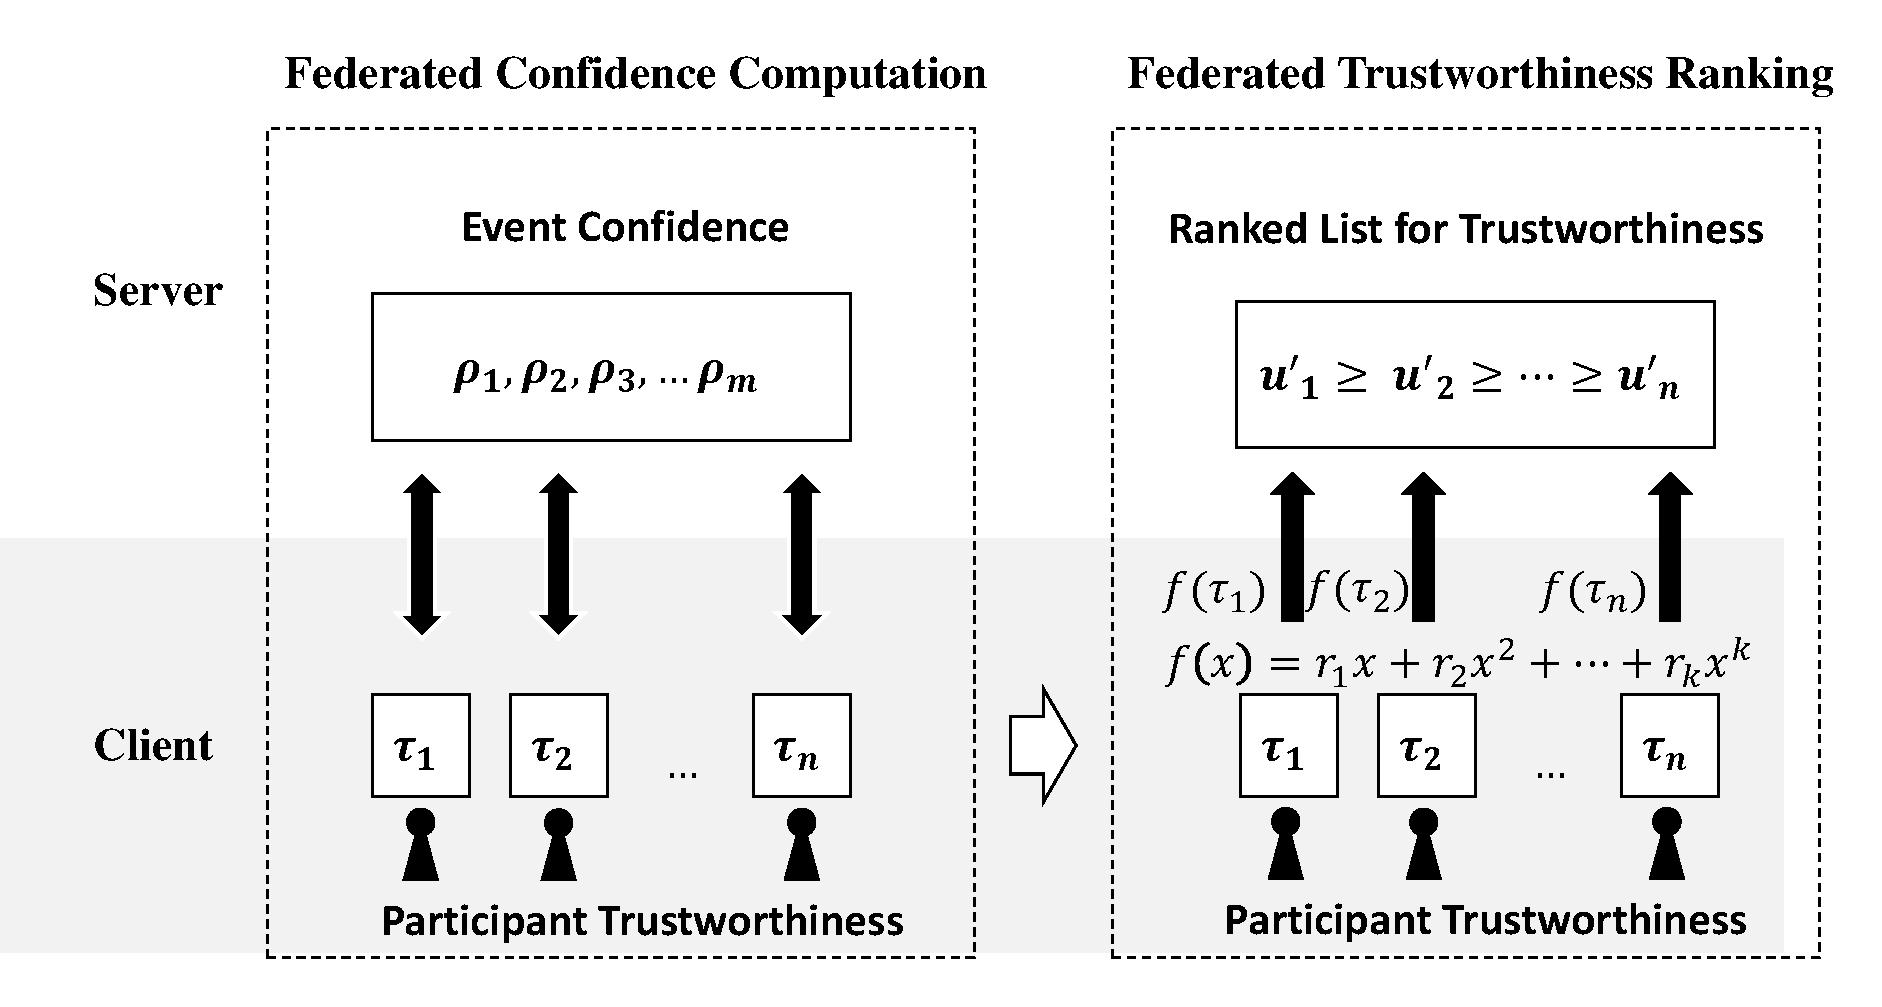
\includegraphics[width=.8\linewidth]{submissions/LeyeWang/fig/overview.pdf}
	\caption{Overview of FedTruthFinder}
	\label{fig:overview}
\end{figure}

Figure~\ref{fig:overview} overviews the workflow of our method \textit{FedTruthFinder}. The general design principle follows the federated learning paradigm \citep{yang2019federated}, which requires the user clients to conduct local computations of their raw data and then upload processed data that do not reveal the user's privacy to the server. With these uploaded privacy-preserving data, the server can still find the aggregate truth of the sensed events, the same as the server receiving the raw sensed data and locations from participants.

By analyzing the original truth discovery algorithm in the previous section, we note that there exist two alternative computation processes: (i) \textit{$\rho$-computation}: updating the confidence $\rho_j$ for each event $e_j$, and (ii) \textit{$\tau$-computation}: updating the trustworthiness $\tau_i$ for each participant $u_i$. In the two computation processes, $\tau$-computation (e.g., Eq.~\ref{eq:tau_function}) can be naturally offloaded to each participant $u_i$'s device, as long as the server sends all the current $\rho_j, \forall e_j$ to the participants. However, $\rho$-computation needs to know each user's sensed data (and locations) and then do aggregation (e.g., sum). This needs a dedicated design to enable the privacy-preserving truth discovery, which will be illustrated in Sec.~\ref{sec:truth_computation}.

Besides, the trustworthiness of each participant's sensed data (i.e., $\tau_i$) is a key metric in crowdsensing organization for participant recruitment and incentive allocation. Hence, we also design a federated privacy-preserving mechanism to rank participants' trustworthiness. Particularly, instead of transferring raw $\tau_i$ to the server, we leverage certain security mechanisms to upload $f(\tau_i)$ to the server, while $f(\tau_i)$ keeps the same ranking orders as $\tau_i$. Particularly, in FedTruthFinder, $f(\tau_i)=r_1\tau_i+r_2\tau_i^2+...+r_k\tau_i^k$, where $r_i>0$.  In this regard, even though the server cannot know the specific $\tau_i$ of each participant $u_i$, the ranked list of participants according to the trustworthiness can still be learned with $f(\tau_i)$. Specifically, during the whole computation process, the server cannot know $r_i$, and each participant will also not know all the $r_i$, so that none of the server or participant can infer other participants' private $\tau_i$. How to compute $f(\tau_i)$ securely will be introduced in Sec.~\ref{sec:trust_ranking}.

\subsection{Key Issues}

\textbf{Issue 1. Privacy-Preserving $\rho$-computation}: \textit{Suppose there are a set of crowdsensing participants $\mathcal U$ and a set of spatial events to sense $\mathcal E$, each participant $u_i (\in \mathcal U)$ with sensed events $\mathcal E_{i,1} (\subseteq \mathcal E)$ and $\mathcal E_{i,0} (\subseteq \mathcal E)$ corresponding to the sensed value being $1$ and $0$, respectively. How to calculate confidence $\rho_j$ for each event $e_j (\in \mathcal E)$ while every participant $u_i$ will not leak $\mathcal E_{i,1}$, $\mathcal E_{i,0}$, and $\mathcal E_{i,1} \cup \mathcal E_{i,0}$ to the server and other participants?}

Some factors need to be carefully considered:

(1) \textbf{Computation}: In $\rho$-computation, the value to share is a complicated equation instead of a single value, and the equation may even be varied depending on the truth discovery algorithm implementation (e.g., Eq.~\ref{eq:rho_function_sum} or Eq.~\ref{eq:rho_function_log}).

(2) \textbf{Network Connection}: In crowdsensing, the network connections of mobile participants may not be always stable. Hence, our mechanism should tolerate the scenario when a few participants lose connections.

(3) \textbf{No Leakage of Task Completion}: For protecting participants' privacy, not only the sensed data but also the completed tasks (i.e., $\mathcal E_{i,1} \cup \mathcal E_{i,0}$) should not be disclosed.

\vspace{+.5em}
\noindent \textbf{Issue 2. Secure Trustworthiness Ranking}: \textit{Suppose there are a set of crowdsensing participants $\mathcal U$ and each participant $u_i (\in \mathcal U)$ has a private trustworthiness score $\tau_i$. How to rank participants according to $\tau_i$ while every participant $u_i$ will not leak $\tau_i$ to the server and other participants?}

Addressing this issue also needs to consider the unstable network connections of participant clients as aforementioned.


\textbf{Remark on security definition}: In this work, we assume that the crowdsensing server and participants are \textit{semi-honest (honest-but-curious)}: they will follow our designed protocol and not maliciously modify the inputs or outputs; however, the server and the participants will try their best to infer others' data from the data that they have received. Besides, our mechanism can defend against \textit{collusion attacks} to a certain extent (i.e., some participants may collude with each other), which we will elaborate on later.

\section{Federated Truth Computation}
\label{sec:truth_computation}

We first introduce a basic scheme for $\rho$-computation in a federated manner assuming no connection loss. Then, we improve the scheme to be against the participants' unpredictable connection loss. %Finally, we theoretically analyze the proposed algorithm.

\subsection{Basic Scheme of $\rho$-Computation with SSS}
\label{sub:basic_rho_computation}

In this section, we propose our basic scheme for the $\rho$-computation problem with the federated learning paradigm leveraging secret sharing. Given a spatial crowdsensing event $e_j$, we first consider $\rho$-computation with the sum function, i.e., Eq.~\ref{eq:rho_function_sum}.

\subsubsection{$\rho$-computation with the sum function.} Our process includes three steps as follows:


\textbf{Step 1 (Share Dispatching)}. Each participant $u_i$ dispatches $d_{ij}$ and $s_{ij}$ with secret sharing to all the $n$ participants ($\mathcal U = \{u_1\cdots u_n\}$), where
\begin{align}
	d_{ij} & =
	\begin{cases}
		\tau_i & \quad\quad e_j \in \mathcal E_{i,1} \\
		0 & \quad\quad e_j \in \mathcal E\setminus \mathcal E_{i,1}
	\end{cases}\\
	s_{ij} &=
	\begin{cases}
		\tau_i & \quad\quad e_j \in \mathcal E_{i,1}\cup \mathcal E_{i,0} \\
		0 & \quad\quad e_j \in \mathcal E\setminus(\mathcal E_{i,1}\cup \mathcal E_{i,0})
	\end{cases}
\end{align}
Specifically, $d_{ij}$ is divided into $n$ shares
$$\{d_{ij}^1,\cdots,d_{ij}^n\}$$
where $d_{ij}^1, \cdots, d_{ij}^{n-1}$ are random numbers and
$$d_{ij}^n = d_{ij} - \sum_{k=1}^{n-1} d_{ij}^k$$
Hence,
$\sum_{k=1}^n d_{ij}^k = d_{ij}$.
Then, $u_i$ sends $d_{ij}^k$ to $u_k$. Similarly, $s_{ij}$ is split to $n$ shares
$$\{s_{ij}^1,\cdots,s_{ij}^n=s_{ij}-\sum_{k=1}^{n-1} s_{ij}^k\}$$
and $u_k$ receives $s_{ij}^k$ from $u_i$.

\textbf{Step 2 (Client Summation)}. For each event $e_j$, an participant $u_k$ uploads $\hat d_{j}^k=\sum_{i=1}^n d_{ij}^k$ and $\hat s_{j}^k = \sum_{i=1}^n s_{ij}^k$ to the server.

\textbf{Step 3 (Server Aggregation)}. After receiving $\hat d_{j}^k$ and $\hat s_{j}^k$ from $\forall u_k \in \mathcal U$, the server can add them together:
\begin{align}
	d_j & = \sum_{k=1}^n \hat d_{j}^k = \sum_{k=1}^n\sum_{i=1}^n d_{ij}^k = \sum_{i=1}^n \sum_{k=1}^n d_{ij}^k = \sum_{i=1}^n d_{ij} \\
	s_j & = \sum_{k=1}^n \hat s_{j}^k = \sum_{k=1}^n\sum_{i=1}^n s_{ij}^k = \sum_{i=1}^n \sum_{k=1}^n s_{ij}^k = \sum_{i=1}^n s_{ij}
\end{align}
Then, $\rho_j$ is computed as:
\begin{equation}
	\rho_j = \frac{d_j}{s_j}
\end{equation}


\subsubsection{$\rho$-computation with the logistic function.} The computation process with the logistic function is not much different from the one with the summation function. Actually, for the event $e_j$, we only need to modify $d_{ij}$ to:
 \begin{align}
 	d_{ij} & =
 	\begin{cases}
 		-\ln(1-\tau_i) & e_j \in \mathcal E_{i,1} \\
 	    \ln (1-\tau_i) & e_j \in \mathcal E_{i,0}\\
 		0 & e_j \in \mathcal E\setminus(\mathcal E_{i,1}\cup \mathcal E_{i,0})
 	\end{cases}
 \end{align}
Besides, we do not need $s_{ij}$, so every participant $u_k$ only receives $d_{ij}^k$ from other $u_i \in \mathcal U$. Finally, in Step 3, we can compute $\rho_j$ as:
\begin{equation}
	\rho_j = (1+e^{-d_j})^{-1}
\end{equation}

\textbf{Remark on our novelty}. In our $\rho$-computation for an event $e_j$, the participant $u_i$ who has not sensed $e_j$ also needs to upload data to the server, e.g., $d_{ij}=s_{ij}=0$ for the sum function. As $d_{ij}$ and $s_{ij}$ are sent by secret shares, the other participants and the server would not know whether $u_i$ senses $e_j$ or not. In comparison, prior studies usually assume that participants send only the data of their sensed events, which may disclose user privacy from event information (e.g., event locations) \citep{Miao2015CloudEnabledPT,Miao2017ALP,Miao2019PrivacyPreservingTD,Zheng2018LearningTT,Zheng2020PrivacyAwareAE,Zhang2021ReliableAP}.

\subsection{Connection Robustness Improvement}

The basic scheme can learn $\rho_j$ in an ideal environment when all the participants are always online. In practice, participants move around and their network connections are often sporadic. This inspires us to make three improvements to the basic scheme design.

\subsubsection{Bias-avoidance adaptive truth updating.}
\label{sub:adaptive_truth_updating}
While participants may drop during the iterative truth discovery process due to bad connections, the original event confidence updating function would be ineffective. Specifically, if $u_i$ loses the connection at the $k^{th}$ iteration, $u_i$'s data would not be considered in the $\rho$-computation (e.g., Eq.~\ref{eq:rho_function_sum}) from then on. This leads to unreliable $\rho_j$ as the finally alive participants dominate the results. To address this pitfall, we propose an adaptive updating function for $k^{th}$ iteration's $\rho_{j,k}$ as,
\begin{equation}
	\rho_{j,k} = w_k F_\rho + (1-w_k) \rho_{j,k-1}
	\label{eq:rho_adaptive_update}
\end{equation}
where $F_\rho$ is an original event confidence updating function (e.g., sum and logistic). With Eq.~\ref{eq:rho_adaptive_update}, the data contribution of the participants who drop at the $k^{th}$ iteration can still be kept (by $\rho_{j,k-1}$) to avoid the truth bias toward alive participants. $w_k$ can be set as,
\begin{equation}
	w_k = (\frac{|\mathcal U_{alive,k}|}{|\mathcal U|})^\alpha
	\label{eq:adaptive_weight}
\end{equation}
where $\mathcal U_{alive,k}$ is the alive participants at the $k^{th}$ iteration. When alive participants decrease with more iterations, $w_k$ becomes smaller, reflecting that fewer participants should occupy lower weights. From our experiments, we find that $\alpha=3$ is a proper setting.

\subsubsection{Server-coordinated communication structure.}
\label{subsub:server_coordination}

In Sec.~\ref{sub:basic_rho_computation}, we assume that one participant $u_i$ can establish a secure communication channel with every other participant $u_k$ so as to transfer the secret share $d_{ij}^k$ and $s_{ij}^k$. Hence, each participant needs to establish $n-1$ channels with others. Considering the sporadic property of the mobile connections, this may not be easy for a participant to keep so many channels stable in practice. To alleviate this issue, we convert the peer-to-peer communication structure to a server-coordinated one. In the server-coordinated structure, every participant first transmits all the data to the server, and then the server dispatches the desired data to the corresponding participant. In this way, each participant  needs to establish \textit{only one} secure channel to the server.

To ensure that the transmitted data will not be directly observed by the server, we leverage a public-key encryption system to encrypt the data before the transmission. In particular, each participant $u_i$ first generates a pair of keys, the public key $pk_i$ and the private key $sk_i$. The public key $pk_i$ is sent to all the other participants (e.g., through the server) at the beginning of the crowdsensing campaign. For details, readers can refer to \citet{Bonawitz2017PracticalSA}.

Then, for computing $\rho_j$, each participant $u_i$ first transmits $E_i = \{\textit{Encrypt}(d_{ij}^k, pk_k)| k = 1\cdots n\}$ to the server.\footnote{If $s_{ij}$ is needed (e.g., for the sum function), it can be encoded in $E_i$ same as $d_{ij}$.} After receiving $n$ participants' $E_i$, the server re-organizes the received data and sends $\hat E_k = \{\textit{Encrypt}(d_{ij}^k, pk_k)| i = 1\cdots n\}$ to each participant $u_k$. Afterward, $u_k$ decrypts the received data with her private key, obtains $\{d_{ij}^k| i = 1 \cdots n\}$, and then uploads $\hat d_j^k = \sum_i d_{ij}^k$ to the server. The server can then recover $d_j = \sum_i d_{ij}$ from participants' uploaded  $\hat d_j^k$ and computes $\rho_j$ accordingly.

\subsubsection{$(t,n)$-Shamir secret sharing (SSS)} While the server-coordinated communication structure reduces the burden of secure channel establishing for mobile participants. It may still fail if a user loses the connection during the campaign and cannot link back. For example, suppose a participant $u_i$ has sent $E_i$ to the server and then quit the crowdsensing campaign (e.g., $u_i$'s mobile device runs out of battery). Then, in Step 3, the server will not be able to receive $\hat d_j^i$ from $u_i$, and thus cannot recover $d_j$.

To address this pitfall, in practical deployment, we can leverage the threshold secret sharing method proposed by Shamir \citep{shamir1979share}, namely \textit{$(t,n)$-Shamir secret sharing (SSS)}. With $(t,n)$-SSS, the server only needs to receive $t\ (t\le n)$ participants' $\hat d_j^i$ for recovering $d_j$. In particular, to leverage $(t,n)$-SSS to dispatch $d_{ij}$, we first create a $(t-1)$-polynomial:
\begin{equation}
	D_{ij}(x) = d_{ij}+a_{ij1}x+a_{ij2}x^2+\cdots+a_{ijt-1}x^{t-1}
\end{equation}
where $a_{ij1},\cdots, a_{ijt-1}$ are random numbers selected by $u_i$. Then, $u_i$ dispatches $D_{ij}(k)$ to $u_k$. If we obtain more than $t$ participants' $D_{ij}(k)$, according to linear algebra, we can infer $d_{ij}$.

Similar to Step 2 of our basic scheme, $\hat d_j^k = \sum_{i} D_{ij}(k)$ is uploaded to the server by each $u_k$. Then, in Step 3, after receiving more than $t$ participants' $\hat d_j^k$, the server will be able to infer $d_j = \sum_{i} d_{ij}$ according to the \textit{additive homomorphism property} of SSS \citep{shamir1979share}.

\textbf{Remark on our novelty}. In the truth discovery part, the key advantage of our mechanism beyond literature is its robustness against connection loss. Preliminary privacy-preserving truth discovery papers rarely consider the connection loss issue \citep{Miao2017ALP}. Some work tries to deal with drop-out users by letting alive participants send extra information \citep{Zhang2021ReliableAP,Wang2021AST}; however, when the connection condition is so bad that certain alive participants again lose connections during the extra information communication, this process would be uncontrolled and time-consuming. Recent work also adopts SSS to enhance connection robustness \citep{Xu2019EfficientAP}. The basic idea is using the double-masking secure aggregation algorithms proposed by \citet{Bonawitz2017PracticalSA}, and every participant needs \textit{two} connections to do event confidence computation for one iteration. In comparison, our mechanism only needs every participant to connect \textit{once} for one iteration of computation. Our numerical experiments (Sec.~\ref{sec:numeric_analysis}) will show that this connection reduction can lead to a significantly difference in the algorithm success probability (e.g., increasing the success probability from $1\%$ to $99\%$ under certain conditions).


\subsection{Theoretical Analysis}
\label{sub:theoretical_analysis_1}


\subsubsection{Correctness} The process to calculate $\rho_i$ in FedTruthFinder follows the original algorithm shown in Sec.~\ref{sec:preliminary}. Hence, we can obtain the same aggregate truth results as the original algorithm, as long as the SSS scheme is valid. In this regard, the correctness of our algorithm is theoretically guaranteed.


\subsubsection{Robustness to Connection Loss \& Security}
Setting $t$ to a small value allows our mechanism to tolerate more users dropping the campaign due to connection losses. Meanwhile, a small $t$ reduces the security level of our mechanism --- if $t$ participants collude with each other, they can recover the other participants' sensed data and locations, leading to privacy leakage.

\textbf{Theorem 4.1}. If there are $\le n-t$ participants losing the connection in one iteration of $\rho$-computation, the server can learn the event confidence $\rho_j$.

\textbf{Theorem 4.2}. If $t' (<t)$ semi-honest users collude with each other, they cannot infer any other users' secret information.

The two theorems hold based on the property of $(t, n)$-SSS.

\subsubsection{Complexity}
We analyze the algorithm from both communication and computation complexity perspectives. Particularly, since the participant clients are more sensitive to the communication and computation overhead, our current analysis focuses on the client side, while the server part analysis is similar.

\textbf{Communication Complexity - $O(nn_e)$}. For each participant client, she needs to transfer $n$ share pieces of the secret to the other participants and receive the corresponding shares from every other participant, so the complexity is $O(n)$ for one event. Suppose there are $n_e$ events, the total communication complexity is $O(nn_e)$.

\textbf{Computation Complexity - $O(nn_e)$}. Each client needs to do two local computation processes. The first process is to generate the random coefficients for $(t,n)$-SSS and calculate the secret shares sent to all the other participants (Step 1), which is $O(nn_e)$. The second process is to do local summation (Step 2), which is also $O(nn_e)$. Hence, the total computation complexity is $O(nn_e)$.
